%
% This is a borrowed LaTeX template file for lecture notes for CS267,
% Applications of Parallel Computing, UCBerkeley EECS Department.
%

\documentclass[twoside]{article}
\usepackage{titlesec}
\setlength{\oddsidemargin}{0.25 in}
\setlength{\evensidemargin}{-0.25 in}
\setlength{\topmargin}{-0.6 in}
\setlength{\textwidth}{6.5 in}
\setlength{\textheight}{8.5 in}
\setlength{\headsep}{0.75 in}
\setlength{\parindent}{0 in}
\setlength{\parskip}{0.1 in}


%
% ADD PACKAGES here:
%

\usepackage{amssymb}	% Already loads amsfonts
\usepackage{amsthm}
\usepackage{graphicx}
\usepackage{mathtools}	% Already loads amsmath
\usepackage{hyperref}
\usepackage{enumitem}
\usepackage{clrscode3e}  % for typesetting pseudocode
\usepackage{ulem}
\usepackage[usenames,dvipsnames]{xcolor}
\usepackage{soul}
\usepackage{cancel}

% Tikz and setup
\usepackage{tikz}
\usepackage{tikz-cd}
\usetikzlibrary{intersections, angles, quotes, calc, positioning}
\usetikzlibrary{arrows.meta}
\usepackage{pgfplots}
\pgfplotsset{compat=1.13}


\tikzset{
    force/.style={thick, {Circle[length=2pt]}-stealth, shorten <=-1pt}
}

%
% The following commands set up the lecnum (lecture number)
% counter and make various numbering schemes work relative
% to the lecture number.
%
\newcounter{lecnum}
\renewcommand{\thepage}{\thelecnum-\arabic{page}}
\renewcommand{\thesection}{\thelecnum.\arabic{section}}
\renewcommand{\theequation}{\thelecnum.\arabic{equation}}
\renewcommand{\thefigure}{\thelecnum.\arabic{figure}}
\renewcommand{\thetable}{\thelecnum.\arabic{table}}

%
% The following macro is used to generate the header.
%
\newcommand{\lecture}[5]{
   \pagestyle{myheadings}
   \thispagestyle{plain}
   \newpage
   \setcounter{lecnum}{#2}
   \setcounter{page}{1}
   \noindent
   \begin{center}
   \framebox{
      \vbox{\vspace{2mm}
    \hbox to 6.28in { {\bf #1
	\hfill} }
       \vspace{4mm}
       \hbox to 6.28in { {\Large \hfill Lecture #2: #3  \hfill} }
       \vspace{2mm}
       \hbox to 6.28in { {\it Lecturer: #4 \hfill Scribe: #5} }
      \vspace{2mm}}
   }
   \end{center}
   \markboth{Lecture #2: #3}{Lecture #2: #3}
   \vspace*{4mm}
}
\renewcommand{\cite}[1]{[#1]}
\def\beginrefs{\begin{list}%
        {[\arabic{equation}]}{\usecounter{equation}
         \setlength{\leftmargin}{2.0truecm}\setlength{\labelsep}{0.4truecm}%
         \setlength{\labelwidth}{1.6truecm}}}
\def\endrefs{\end{list}}
\def\bibentry#1{\item[\hbox{[#1]}]}

\newcommand{\fig}[3]{
			\vspace{#2}
			\begin{center}
			Figure \thelecnum.#1:~#3
			\end{center}
	}

% Colored theorem styles
\makeatother
\usepackage{thmtools}
\usepackage[framemethod=TikZ]{mdframed}
\mdfsetup{skipabove=1em,skipbelow=0.5em}

\declaretheoremstyle[
    headfont=\bfseries\sffamily\color{ForestGreen!70!black}, bodyfont=\normalfont,
    mdframed={
        linewidth=2pt,
        rightline=false, topline=false, bottomline=false,
        linecolor=ForestGreen, backgroundcolor=ForestGreen!5,
    },
    spaceabove=8pt
]{thmgreenbox}

\declaretheoremstyle[
    headfont=\bfseries\sffamily\color{NavyBlue!70!black}, bodyfont=\normalfont,
    mdframed={
        linewidth=2pt,
        rightline=false, topline=false, bottomline=false,
        linecolor=NavyBlue, backgroundcolor=NavyBlue!5,
    },
    spaceabove=8pt
]{thmbluebox}

\declaretheoremstyle[
    headfont=\bfseries\sffamily\color{NavyBlue!70!black}, bodyfont=\normalfont,
    mdframed={
        linewidth=2pt,
        rightline=false, topline=false, bottomline=false,
        linecolor=NavyBlue
    },
    spaceabove=8pt
]{thmblueline}

\declaretheoremstyle[
    headfont=\bfseries\sffamily\color{RawSienna!70!black}, bodyfont=\normalfont,
    mdframed={
        linewidth=2pt,
        rightline=false, topline=false, bottomline=false,
        linecolor=RawSienna, backgroundcolor=RawSienna!5,
    },
    spaceabove=8pt
]{thmredbox}

\declaretheoremstyle[
    headfont=\bfseries\sffamily\color{RawSienna!70!black}, bodyfont=\normalfont,
    numbered=no,
    mdframed={
        linewidth=2pt,
        rightline=false, topline=false, bottomline=false,
        linecolor=RawSienna, backgroundcolor=RawSienna!1,
    },
    qed=\qedsymbol,
    spaceabove=8pt
]{thmproofbox}

\declaretheoremstyle[
    headfont=\bfseries\sffamily\color{NavyBlue!70!black}, bodyfont=\normalfont,
    numbered=no,
    mdframed={
        linewidth=2pt,
        rightline=false, topline=false, bottomline=false,
        linecolor=NavyBlue, backgroundcolor=NavyBlue!1,
    },
    spaceabove=8pt
]{thmexplanationbox}

% Use these for theorems, lemmas, proofs, etc.
\theoremstyle{definition}
\declaretheorem[style=thmgreenbox, name=Definition, numberwithin=lecnum]{definition}
\declaretheorem[style=thmbluebox, numbered=no, name=Example]{example}
\declaretheorem[style=thmredbox, name=Proposition, numberwithin=lecnum]{proposition}
\declaretheorem[style=thmredbox, name=Theorem, numberwithin=lecnum]{theorem}
\declaretheorem[style=thmredbox, name=Lemma, sibling=theorem]{lemma}
\declaretheorem[style=thmredbox, name=Corollary, sibling=theorem]{corollary}
% \newtheorem{theorem}{Theorem}[lecnum]
% \newtheorem{lemma}[theorem]{Lemma}
% \newtheorem{claim}[theorem]{Claim}
% \newtheorem{corollary}[theorem]{Corollary}
% \newtheorem{definition}[theorem]{Definition}
\declaretheorem[style=thmblueline, numbered=no, name=Remark]{remark}
\declaretheorem[style=thmblueline, numbered=no, name=Conjecture]{conjecture}
\renewenvironment{proof}{{\bf \textit{Proof.}}}{\hfill\rule{2mm}{2mm}}
\makeatletter


% **** IF YOU WANT TO DEFINE ADDITIONAL MACROS FOR YOURSELF, PUT THEM HERE:

\renewcommand\Pr{\mathbb{P}}
\newcommand\Ex{\mathbb{E}}

\newcommand\N{\mathbb{N}}
\newcommand\Z{\mathbb{Z}}
\newcommand\Q{\mathbb{Q}}
\newcommand\R{\mathbb{R}}
\newcommand\C{\mathbb{C}}
\newcommand\F{\mathbb{F}}

\DeclarePairedDelimiter\ceil{\lceil}{\rceil}
\DeclarePairedDelimiter\floor{\lfloor}{\rfloor}
\DeclarePairedDelimiter\anglebrac{\langle}{\rangle}

\newcommand{\divides}{\mathrel{\mid}}
\newcommand{\notdivides}{\mathrel{\nmid}}

\begin{document}
\lecture{MATH453 Elementary Number Theory}{2}{Congruence and The Division Algorithm}{Bruce Berndt}{Kevin Gao}

\section{Congruence and Sum of Two Squares}

Recall that $a \equiv b \mod c$ if and only if $c \divides (a-b)$. 

If $p \equiv 1 \mod 4$, we will show that $p = a^2 + b^2$ for some integers $a$ and $b$. Such pair of $a,b$ where $a,b \in \Z$ is called a \textit{\textbf{lattice point}}.

\begin{theorem}[Fermat's theorem on sum of two squares]
    An odd prime $p$ can be expressed as $p = x^2 + y^2$ with integers $x$ and $y$ if and only if $p \equiv 1 \mod 4$.
\end{theorem}

Let $r_2(n)$ denote the number of representations of $n$ as a sum of two squares. We would like to study the behavior of $\sum_{n \leq x} r_2(n)$.

We start with \textbf{Gauss's attempt} in trying to bound $\sum_{n \leq x} r_2(n)$. As we can see, each lattice point can be represented as the coordinate $(m,n)$ of a point on a plane. If we draw a circle with radius $r$, then all lattice points within the circle have the property
$$
m^2 + n^2 \leq r^2
$$
Then, the problem of bounding $\sum_{n\leq x}r_2(n)$ for some $x$ is the same as finding the number of lattice points within the circle centered at $(0,0)$ with radius $\sqrt{x}$. Because of this, the problem is also known as \textit{\textbf{Gauss circle problem}}.

\begin{figure}[htbp]
    \centering
    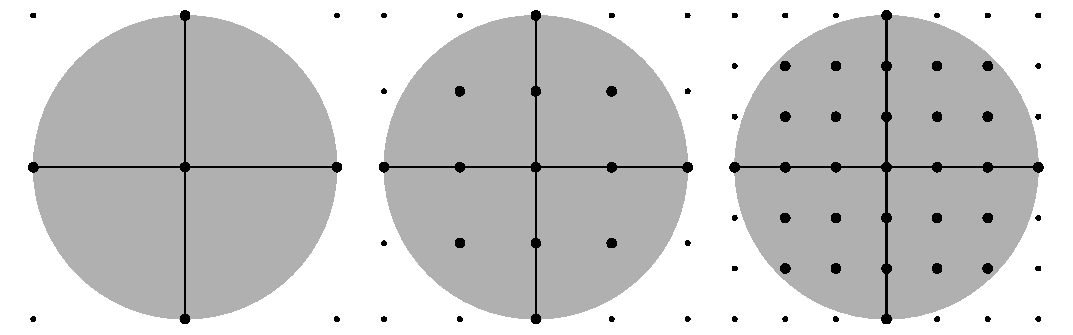
\includegraphics[width=0.5\linewidth]{figures/GausssCircleProblem.pdf}
    \caption{Gauss's circle problem}
    \label{fig:gauss-circle-prob}
\end{figure}

\begin{theorem}[Gauss's solution]
    $$
    \sum_{n \leq x} r_2(n) = \pi x + O(\sqrt{x}) = \pi x + \underbrace{E(x)}_{\text{error term}}
    $$
    So, $E(x) \in O(x^{1/2})$.
\end{theorem}

\begin{proof}
    We associate each representation of a number as two squares with a square on the plane, enclosed within the circle of radius $\sqrt{x}$.

    Then, the number of such lattice points is bounded above by the area of the larger circle and bounded below by the smaller circle.
    $$
    \pi(\sqrt{x} - 1)^2 \leq \sum_{n \leq x}r_2(n) \leq \pi(\sqrt{x} + 1)^2
    $$
    \begin{figure}[htbp]
        \centering
        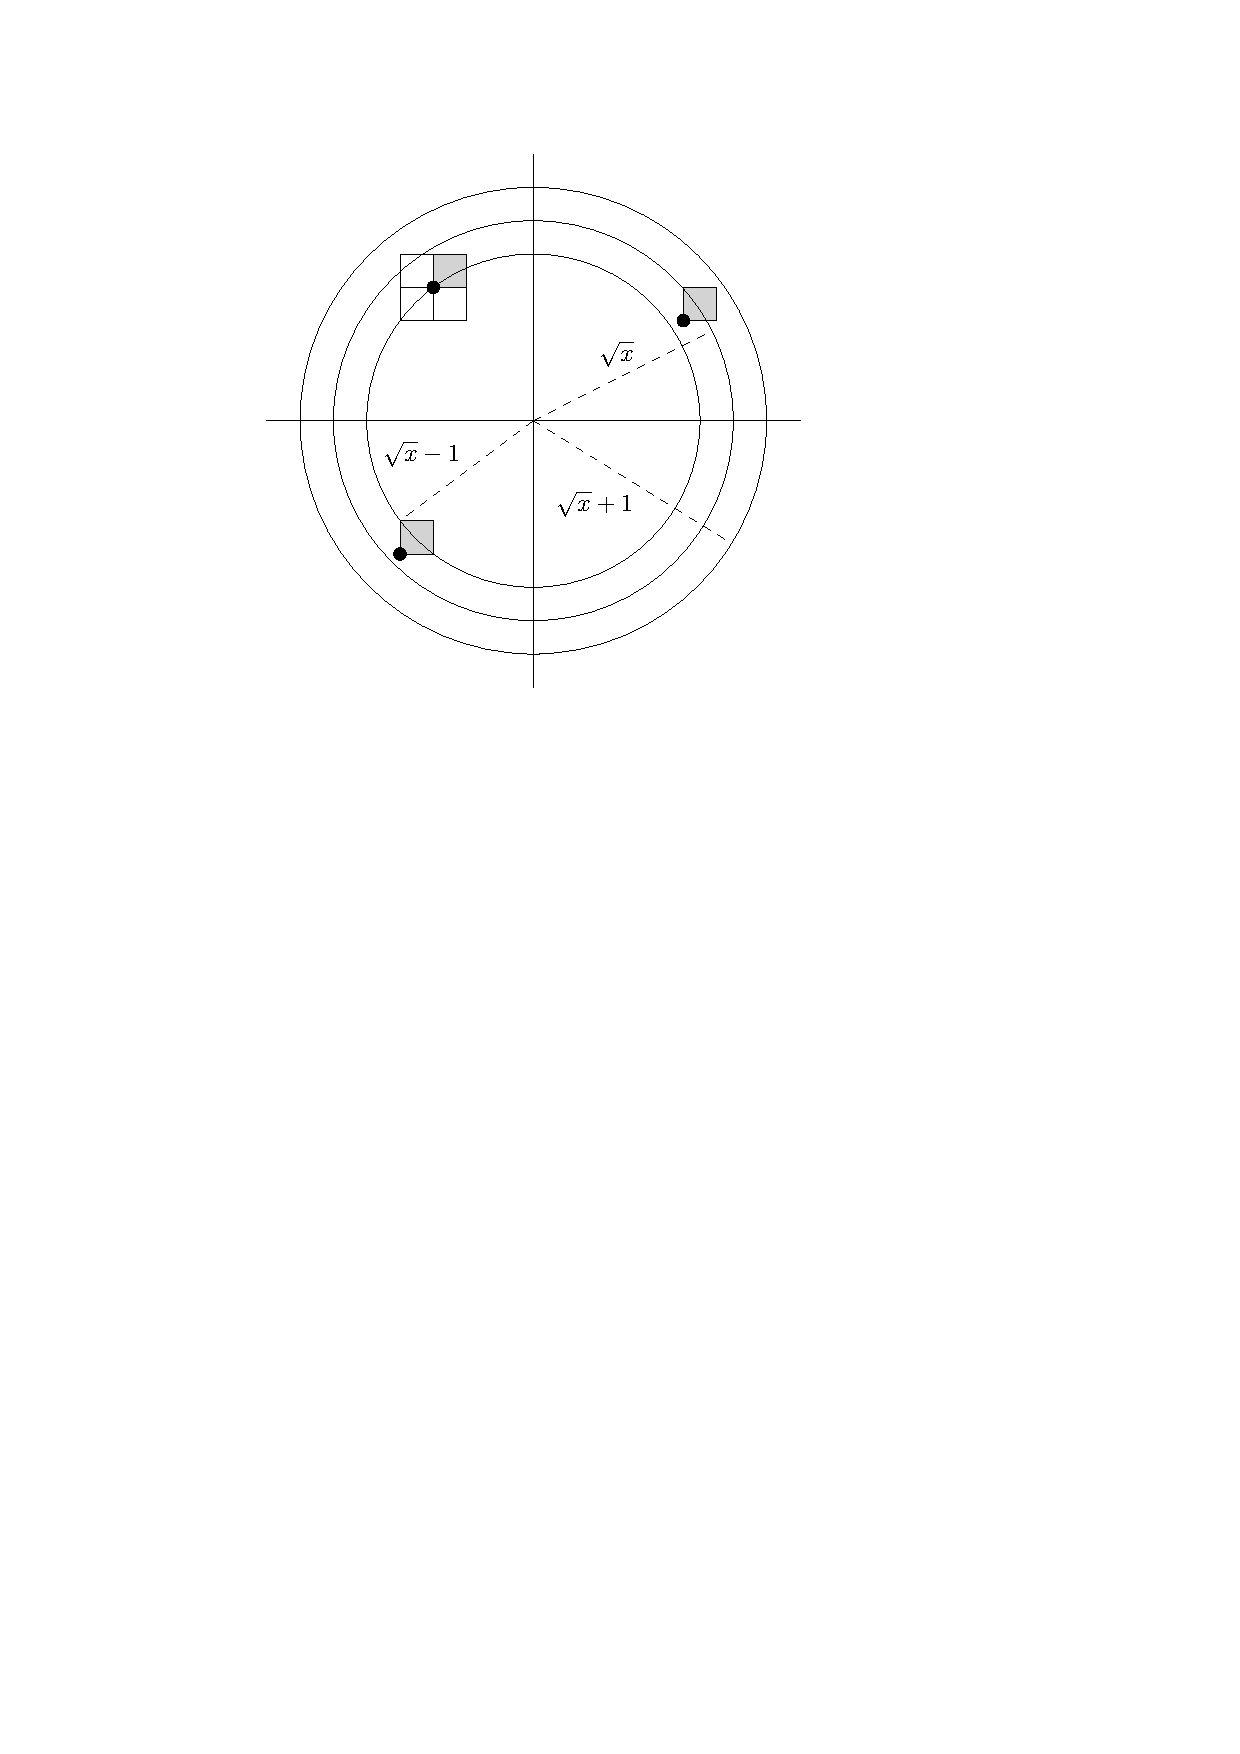
\includegraphics[width=.4\linewidth]{figures/gauss-circle-area.pdf}
        \caption{Using area to bound the number lattice points.}
        \label{fig:gauss-circle-area}
    \end{figure} 
    We can further rearrange this to get
    $$
    \pi(x - 2\sqrt{x+1}) \leq \sum_{n \leq x} r_2(n) \leq \pi(x + 2\sqrt{x} + 1)
    $$
    Then, $\sum_{n\leq x}r_2(n) = \pi x + O(\sqrt{x})$. 
\end{proof}

Over the years, there have been numerous improvements on bounding the error term.

\begin{theorem}[Sierpinski 1906]
    $$
    \sum_{n \leq x} r_2(n) = \pi x + O(x^{1/3})
    $$
\end{theorem}

\section{Integer Partition}

Next, we will consider the integer partition. A \textit{\textbf{partition}} of an integer $n \in \Z^+$ is one way of representing $n$ as a sum of \textbf{more than one} (possibly repeating) integers.

We define $P(n)$ to be the number of ways of writing $n \in \Z^+$ as a sum of positive integers (ways to partition $n$).

For example, $P(4) = 5$ because $4 = 3+1 = 2+2 = 2+1+1 = 1+1+1+1$. Note that $4$ itself does not count since we need at least 2 integers for it to be a valid partition.

\begin{conjecture}[Ramanujan's Conjecture on Integer Partition]
    $P(5n + 4) \equiv 0 \mod 5$, $P(7n + 5) \equiv 0 \mod 7$, $P(11n + 6) \equiv 0 \mod 11$.
\end{conjecture}

\section{Division Algorithm}

\subsection{Propositions About Division}

Before we talk about the division algorithm, we first introduce some useful propositions about division.

\begin{proposition}
    $a \divides b$ and $b \divides c$ $\implies$ $a \divides c$. 
\end{proposition}

\begin{proof}
    The proof is straightforward from the definition of the division relation.

    Since $a \divides b$, $\exists c_1 \in \Z.\, b = c_1a$. Similarly, $\exists c_2 \in \Z.\, c = c_2 b$ since $b \divides c$. We can then rewrite $c$ as $c = c_2 b = c_1c_2a = (c_1c_2)a$. Since $c_1$ and $c_2$ are all integers, $c_1c_2$ is also an integer. Then, by definition, $a \divides c$.
\end{proof}

\begin{proposition}
    If $c \divides a$ and $c \divides b$, then $\forall m,n \in \Z.\, c \divides (ma+nb)$.
\end{proposition}

\begin{proof}
    Again, this is immediate from the definition and basic arithmetics.

    Since $c \divides a$, $\exists c_1 \in \Z.\, a = c_1c$. Since $c \divides b$, $\exists c_2 \in \Z.\, b = c_2 c$.

    Let $m,n \in \Z$ be arbitrary. Then, $ma + mb = mc_1c+nc_2c = c(mc_1 + nc_2)$. By definition, $c \divides (ma + mb)$.
\end{proof}

\subsection{Floor and Ceiling}

\begin{definition}[Floor]
    The floor of $x$, denoted $\floor{x}$, is the greatest integer less than or equal to $x$.
\end{definition}

Similarly, we define the ceiling as follows

\begin{definition}[Ceiling]
    The ceiling of $x$, denoted $\ceil{x}$, is the smallest integer greater than or equal to $x$.
\end{definition}

\begin{remark}
    In his lecture notes, Professor Berndt used $[\cdot]$ for floor. I decided to use the more standard notation in my notes to avoid confusion.
\end{remark}

\begin{lemma} \label{lem:div-algo-lem1}
    For $x \in \R$, $x-1 < \floor{x} \leq x$.
\end{lemma}

\begin{proof}
    By contradiction. Suppose not, then there exists some $x \in \R$ such that $x-1 \geq \floor{x}$. Take such $x$ and add 1 to both sides of the inequality, yielding $x \geq \floor{x} + 1$. But by definition, $\floor{x}$ is the greatest integer less than or equal to $x$. The fact that $\floor{x}+1$, which is strictly greater than $\floor{x}$, is also less than or equal to $x$ contradicts the definition of floor. Therefore, the original lemma holds. 
\end{proof}

\subsection{The Division Algorithm}

The \textbf{division algorithm} is also known as the \textbf{quotient remainder theorem}. The statement is as follows.

\begin{theorem}[The Division Algorithm]
    Let $a,b \in \Z$ such that $b > 0$. Then, there exists unique $q,r \in \Z$ such that $a = bq + r$ and $0 \leq r < b$.    
\end{theorem}

\begin{proof}
    We divide the proof into two parts: existence and uniqueness. We first prove \textbf{existence} by construction.

    Take $q = \floor{a/b}$ and $r = a - b \floor{a/b}$. Then, we have
    $$
    a = b \left\lfloor \frac{a}{b} \right\rfloor + r
    $$
    This proves that $a = bq + r$. Next, we show that $0 \leq r < b$. By Lemma \ref{lem:div-algo-lem1}, 
    $$
    \frac{a}{b} - 1 < \left\lfloor \frac{a}{b} \right\rfloor \leq \frac{a}{b}
    $$
    Since $b > 0$, we can multiply both sides by $b$, yielding
    $$
    a - b < \left\lfloor \frac{a}{b} \right\rfloor b \leq a
    $$
    Mutiply by -1 and reversing the signs, and then add $a$ to both sides
    $$
    \begin{aligned}
        b - a &> - \left\lfloor \frac{a}{b} \right\rfloor b &\geq -a \\
        b &> - \left\lfloor \frac{a}{b} \right\rfloor b + a &\geq 0
    \end{aligned}
    $$
    Since $r = a - b \floor{a/b}$, by substitution, $b > r \geq 0$. This proves the existence of such $q,r$.

    Next, we prove the \textbf{uniqueness} of such $q$ and $r$ by contradiction. Suppose for contradiction that there exists some $q' \neq q$ and $r' \neq r$ such that $a = bq' + r'$ and $0 \leq r' < b$. Then,
    $$
    a - a = 0 = b(q - q') + (r - r')
    $$
    $|r - r'| < b$ because both $r < b$ and $r' < b$. WLOG, suppose $r' > r$. Then, $r' - r = b(q' - q)$ by rearranging the previous inequality. This implies that $r' - r$ is a multiple of $b$. But since $r' - r$ is strictly less than $b$,
    $$
    0 \leq r' - r < b
    $$
    $r'-r$ must be 0. This contradicts the assumption that $r \neq r'$. Similarly, $q = q'$ since $r = r'$, which is also a contradiction.
\end{proof}

\end{document}